%author: Simone Notargiacomo, Lorenzo Tavernese, Ibrahim Khalili
%date: 19 Giugno 2008
\documentclass[a4paper,italian,12pt]{beamer}
\usepackage[utf8]{inputenc}
\usepackage[italian,english]{babel}
\usepackage[T1]{fontenc}
\usepackage{beamerthemesplit}
\usepackage{graphicx}
\usepackage{float}
\usepackage{xcolor}
\usepackage{times}
\usepackage{colortbl}

\setbeamercolor{uppercol}{fg=black,bg=white}
\setbeamercolor{lowercol}{fg=black,bg=blue}

%\usepackage{tikz}
%\usetikzlibrary{arrows}
%\tikzstyle{block}=[draw opacity=0.7,line width=1.4cm]

%\setbeamercolor{sidebar right}{bg=black!15}
%\setbeamercolor{structure}{fg=blue}
%\setbeamercolor{author}{parent=structure}

\usetheme{Antibes}
\useoutertheme{smoothbars}
%\useoutertheme{infolines}
%\usecolortheme{rose}
\useinnertheme{circles}

\title{Ingegneria del Web 07/08}
\institute{Università di Roma Tor Vergata}
\author{Lorenzo Tavernese}
%\logo{
\includegraphics[scale=0.1]{etc/tortellalogo.jpg}}
\date{\today}

\begin{document}
	\begin{frame}
		\titlepage
		\begin{figure}[H]
			\begin{center}
				
\includegraphics[scale=0.4]{etc/tortellalogo.jpg}
			\end{center}
		\end{figure}
	\end{frame}

    \section{Sommario}
	    \frame{\tableofcontents}

	\section{Servent}
		\subsection{Connessione}
			\begin{frame}
				\frametitle{Fake ID vs Real ID}
				\begin{itemize}
					\item Il fake ID serve per la connessione ad un peer di cui si conoscono solo ip e porta.
					\item Il valore massimo dei fake ID è impostato nel conf file.
					\item Il valore massimo viene utilizzato per distinguere i fake ID da quelli reali.
				\end{itemize}
			\end{frame}
			\begin{frame}
				\frametitle{Prima fase}
				\begin{itemize}
					\item Nodo1 invia un pacchetto PING con fake ID al Nodo2.
					\item Il Nodo1 attende la conferma di ricezione.
					\item Il Nodo2 invia la conferma di ricezione.
				\end{itemize}
				\begin{figure}[H]
					\begin{center}
						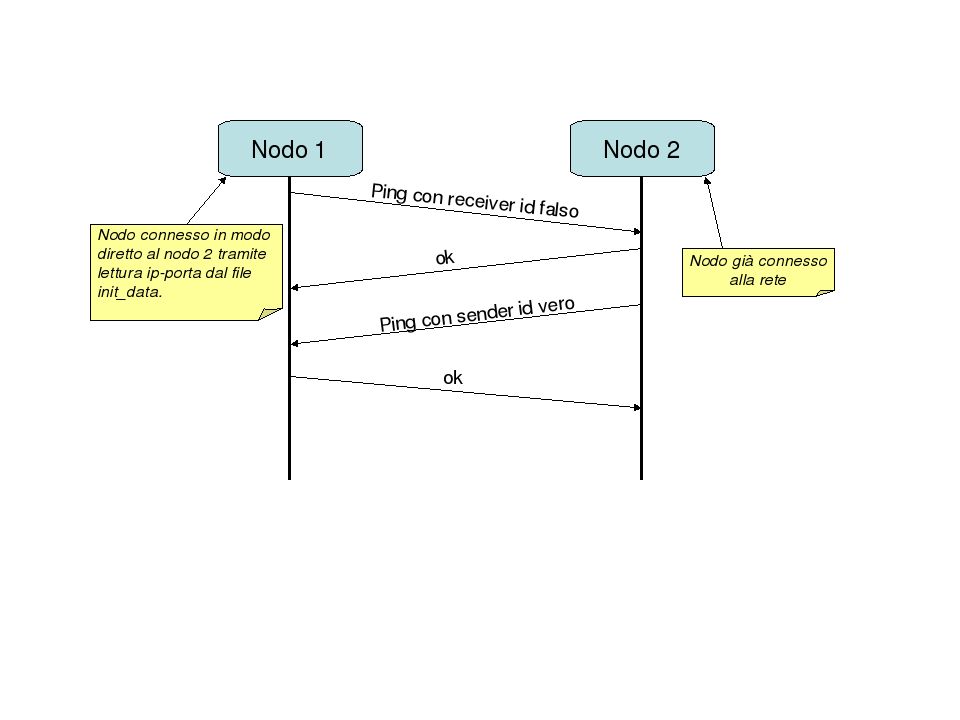
\includegraphics[scale=0.3]{etc/Bootstrap.png}
					\end{center}
				\end{figure}
			\end{frame}
			\begin{frame}
				\frametitle{Seconda fase}
				\begin{itemize}
					\item Il Nodo2 riceve il PING ed invia PING con ID reale.
					\item Il Nodo2 attende la conferma di ricezione.
					\item Il Nodo1 riceve il PING con l'ID reale.
					\item Il Nodo1 invia la conferma di ricezione.
					\item Connessione avvenuta.
				\end{itemize}
				\begin{figure}[H]
					\begin{center}
						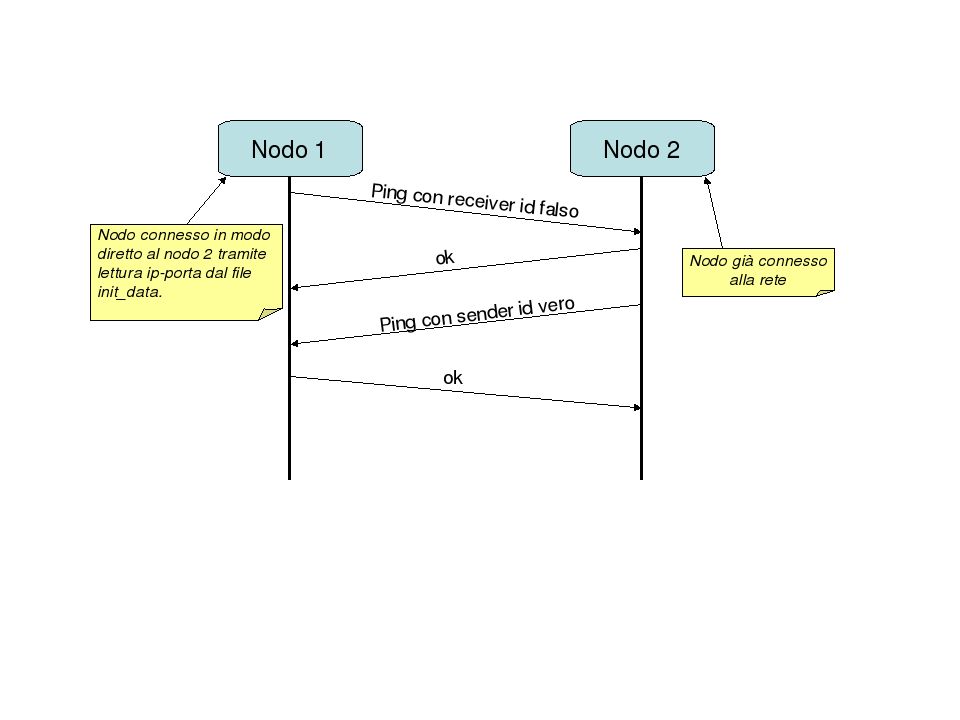
\includegraphics[scale=0.3]{etc/Bootstrap.png}
					\end{center}
				\end{figure}
			\end{frame}

	\section{Applicazione}
		\subsection{Architettura}
			\begin{frame}
				\frametitle{Panoramica}
				\begin{figure}[H]
					\begin{center}
						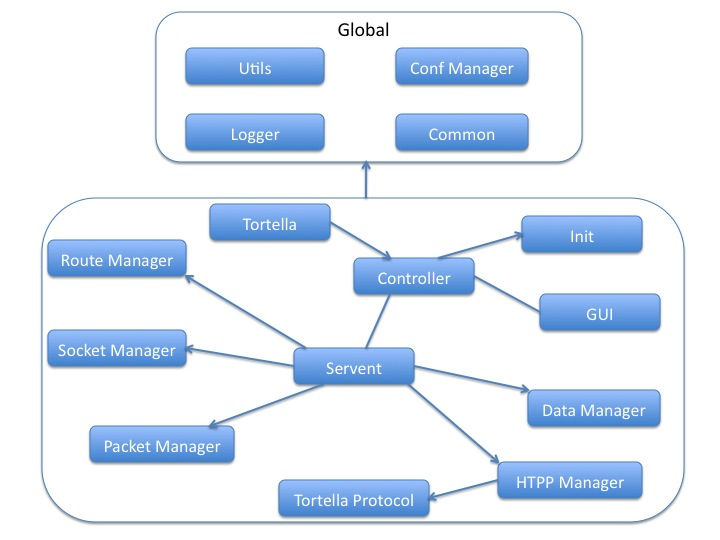
\includegraphics[scale=0.3]{etc/architectural_overview.png}
					\end{center}
				\end{figure}
			\end{frame}
				
		\subsection{Messaggi}
			\begin{frame}
				\frametitle{Descrizione}
				\begin{itemize}
					\item Messaggi inviati direttamente ai peer.
					\item Si evita il flooding poichè le connessioni sono già stabilite.
					\item Possibile sviluppo di messaggi crittografati.
					\item Tipi di messaggi:
					\begin{itemize}
						\item Invio di \textit{private message}.
						\item Invio di messaggi a sottoinsiemi di utenti.
						\item Invio di messaggi a tutta la chat room.
					\end{itemize}
				\end{itemize}
			\end{frame}
			
		\subsection{Gestione pacchetti}
			\begin{frame}
				\frametitle{Invio pacchetti}
				\begin{itemize}
					\item Preparazione struttura dati \texttt{servent\_data} riguardante il peer remoto con cui comunicare.
					\item Inserimento della \texttt{servent\_data} nella coda di richieste.
					\item Il \textit{client thread} estrae la richiesta dalla coda.
					\item Il \textit{client thread} invia il pacchetto al peer specificato.
					\item Il \textit{client thread} attende il pacchetto di conferma ricezione.
					\item Ricevuto il pacchetto lo aggiunge alla coda delle risposte.
					\item Nei livelli superiori si controllano i pacchetti nella coda delle risposte.
				\end{itemize}
			\end{frame}
			\begin{frame}
				\frametitle{Ricezione pacchetti}
				\begin{itemize}
					\item Il \textit{server thread} riceve un pacchetto TorTella.
					\item Controlla la presenza e la coerenza dei dati ricevuti.
					\item Invia il pacchetto di risposta.
					\item In base al tipo di pacchetto effettua delle operazioni specifiche:
					\begin{description}
						\item[Ping:] Se necessario rinvia un Ping al mittente.
						\item[Search:] Rinvia il pacchetto agli altri peer ed un SearchHits al mittente.
						\item[SearchHits:] Rinvia il pacchetto sfruttanto il Backward Routing.
						\item[Join e Leave:] Inoltra il pacchetto in flooding.
					\end{description}
				\end{itemize}
			\end{frame}
		\subsection{Disconnessione}
			\begin{frame}
				\frametitle{Bye e Close}
				\begin{itemize}
					\item Per la disconnessione dai peer si utilizza il pacchetto Bye.
					\item Per la chiusura dei \textit{client thread} si usa il \texttt{CLOSE\_ID}.
					\item Il \textit{server thread} termina alla ricezione del Bye.
				\end{itemize}
			\end{frame}

\end{document}